\scanpage{359}
Cor\hfill EZ 2
\diagram{\begin{tikzcd}
\Sigma_n\arrow[r]&E\Sigma_n=\deleted{\unsure{B(E\Sigma_n)}}\arrow[d,no head]\\
&\unsure{K|\kappa}(\Sigma_n,1)
\end{tikzcd}}
\diagram{\begin{tikzcd}
{}&\ldots\arrow[l,no head]&\Sigma_n\times\Sigma_n\arrow[r,shift left]\arrow[r,shift right]&\Sigma_n
\end{tikzcd}}
\diagram{\begin{tikzcd}
W_n=\mathbb Z E\Sigma_n\arrow[r,"\sim","\text{résol de }\mathbb Z\text{ par des }\Sigma_n\text{-modules \deleted{\unsure{plts}} libres.}"']&\mathbb Z
\end{tikzcd}}

Cor du th
\diagram{\begin{tikzcd}
W_n\arrow[r,"\unsure{?|\sim}"]&\operatorname{Hom}^{\unsure{'|\bullet}}(\deleted{\unsure{\mathbb ZX\otimes\mathbb ZX}}\ \mathbb ZX\times X\times\ldots,\mathbb ZX\otimes\ldots\otimes\mathbb ZX)
\end{tikzcd}}
D'où par adjonction une flèche
\diagram{\begin{tikzcd}
W_n\otimes\mathbb Z(X\times\ldots\times X)\arrow[r,"\lambda"]&\mathbb ZX\otimes\mathbb ZX\ldots\otimes\mathbb ZX
\end{tikzcd}}
(resp.
\diagram{\begin{tikzcd}
W_n\otimes\mathbb ZX\otimes\ldots\otimes\mathbb ZX\arrow[r]&\mathbb Z(X\times\ldots\times X)^\sim
\end{tikzcd}}
)
Ceci exprime l'homotopie-commutativité \unsure{énoncée|annoncée} $+$ haut

\uline{Ex $n=2$}\qquad1) exemple topologique:
\diagram{\begin{tikzcd}
X\times X\arrow[r,"m"]&X\quad\text{\unsure{homotopiq cm}}
\end{tikzcd}}
$\Sigma_2$ équiv
\diagram{\begin{tikzcd}[column sep=large,execute at end picture={\draw (-.8,0) ellipse (2.15 and .4);\draw (3,0) .. controls (3.35,.1) and (3.5,-.1) .. (3.5,-.25);}]
I\times X\times X\arrow[r]&X\arrow[r,dotted,no head]&{}
\end{tikzcd}}
$+$ fort
\diagram{\begin{tikzcd}
\underbrace{E\Sigma_2}\times X^2\arrow[r,maps to]&X\quad\Sigma_2\text{ équiv}\\
E\Sigma_n\times X^n\arrow[r]&X\quad\text{relevant la mult itérée}
\end{tikzcd}}
\unsure{Classiquemen|Classiquement}

$\Sigma_2$ agit sur $S^n$ par action antipodale
\diagram{\begin{tikzcd}
{}\arrow[d,no head]&E\Sigma_2=\varinjlim S^n\\
P^n(\mathbb R)&{}
\end{tikzcd}}
\margin{$x,y$\quad\deleted{$xy=yx$}\quad$xyx^{-1}y^{-1}$}
\diagram{\begin{tikzcd}
S^1\times X^2\arrow[r]\arrow[d,no head]&X\\
S^2\times X^2\arrow[ur,"\Sigma_2\text{-équiv}"']&{}
\end{tikzcd}}
etc\ldots
\figure{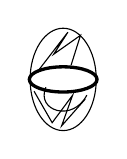
\begin{tikzpicture}
\draw (0,0) ellipse (.42 and .65);
\draw[very thick] (0,0) ellipse (.43 and .16);
\draw (-.31,.12)--(.06,.6)--(-.12,.32)--(.22,.56)--(.1,.18);
\draw (-.37,-.15)--(-.14,-.55)--(.12,-.2)--(-.02,-.59)--(.28,-.25);
\draw (-.22,-.1) .. controls (-.35,-.4) and (.12,-.55) .. (.3,-.2);
\end{tikzpicture}}

\diagram{\begin{tikzcd}[column sep=large]
\deleted{\unsure{E\Sigma_n\times(E\Sigma_j\times X)^n}}\arrow[d]&E(\Sigma_n\unsure{\int|\wr}\Sigma_j)\times(X_1^0\ldots X_j^0)\times X_1^1\ldots X_j^1\times\ldots X_1^n\times\ldots\times X_j^n\arrow[l]\arrow[dd]\\
X^n&\text{?}\\
X&E\Sigma_n\times X^n\arrow[l]
\end{tikzcd}}
\figure{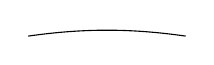
\begin{tikzpicture}\draw (0,0) .. controls (.7,.1) and (1.3,.1) .. (2,0);\end{tikzpicture}}
Cor: les énoncés précédents impliquent que lorsque $X$ est un H esp sat à ce genre de cdn de commutativité à homotopie près,
alors les \unsure{chains|chaînes} $\mathbb ZX$ \unsure{est à}
\diagram{\begin{tikzcd}
\underbrace{W_n}\otimes\mathbb ZX^{\otimes n}\arrow[r,"\Sigma_n\text{ équiv}"]&\mathbb ZX^{\unsure{\sim|\xi}}\arrow[r]&{}
\end{tikzcd}}
t.q. induise la mult de chaine
\diagram{\begin{tikzcd}
\mathbb ZX^{\otimes n}\arrow[r,"\mathrm{EZ}","\text{shuffles}"']&\mathbb Z(X^n)\arrow[r,"\mathbb Z(m)"]&\mathbb ZX
\end{tikzcd}}
\figure{\begin{tikzpicture}\draw (0,0)--(.8,-.03);\end{tikzpicture}}

Constr des opérations de Steenrod:

$A$ un anneau de car $p$
\diagram{\begin{tikzcd}
\mathbb ZX\arrow[r]&{}
\end{tikzcd}}
$\unsure{f}\in\unsure{Z^n|C^n}(X,A)$
\diagram{\begin{tikzcd}
(\widetilde{\mathbb Z}X)\arrow[r,"f"]&A[n]
\end{tikzcd}}
\diagram{\begin{tikzcd}[column sep=small]
W_p\otimes\mathbb Z(X^p)\arrow[r,"\lambda"]\arrow[rrr,bend right=15,no head]&\widehat{\mathbb Z}X^{\otimes p}\arrow[r,"f^{\otimes p}"]&A[n]^{\otimes p}\arrow[r,"\mu"]&A[pn]\\
W_p\otimes\mathbb ZX\arrow[u,"\Delta"]\arrow[urrr,"\Sigma_n\text{ équiv}"']&&&{}
\end{tikzcd}}
\margin{\fbox{\begin{tabular}{ll}cf Steenrod&\uline{p99}\\\uline{Coh ops}&\end{tabular}}}
(avec action triv sur $\mathbb ZX$)
\deleted{$\unsure{W_n\otimes\mathbb ZX}$}
\diagram{\begin{tikzcd}
Pf=\mu\circ f^{\otimes p}\circ\lambda\quad\in{}_{\Sigma_n}H^{pn}(\unsure{\mathbb Z(X^p)},A)\arrow[d]\\
{}_{\Sigma_n}H^{\unsure{pn}}(X,A)
\end{tikzcd}}
\[
(W_n\otimes\mathbb ZX)/\Sigma_n\simeq\mathbb ZX\otimes\mathbb Z\unsure{K|\kappa}(\Sigma_n,1)
\]
$\Sigma_n$
\[
\begin{gathered}
\text{''}\\
H^*(\unsure{K|\kappa}(\Sigma_p)\unsure{\times|\otimes}X,A)\\
\text{''}\\
H^*(\Sigma_p)\otimes_{\mathbb F_p}H^*(X,A)
\end{gathered}
\]
\margin{\unsure{Kunneth|Künneth}}
\mspage{360}
